\chapter{Hash Tables}
\label{ch:hash-tables}

In previous chapters, we have seen how lists can be used to store
multiple values, such as all the students in a class or the books
in a library. Lists provide convenient access to their first element 
and to their remaining elements as a list, so all the elements of a 
list can be processed with a function that can be defined inductively
with a few simple equations.  This is fine when you really do want to 
process all the elements in the list, but what if you're only interested 
in the student with ID \#93574 or Mary Shelley's ``Frankenstein; or, 
The Modern Prometheus''? Computer scientists have designed more convenient
data structures for just these situations, and we'll study one of these
solutions in this chapter. 

\section{Lists and Arrays}

Let's start with a list of states and their capitals, such as
\begin{Verbatim}
( (alabama  montgomery)
  (alaska   juneau)
  (arizona  phoenix)
  ...
  (wyoming  cheyenne) )
\end{Verbatim}
We could use this list to find the capital of any given state with a
function 
\begin{center}
Axioms for capital lookup function
\begin{tabular}{ll}
(capital $s$ nil) = nil  & \{\emph{cap0}\}     \\
(capital $s$ (cons (list $state$ $city$) $caps$)) = city, if $s=state$ & \{\emph{cap1}\} \\
(capital $s$ (cons (list $state$ $city$) $caps$)) = (capital $s$ $caps$), if $s \ne state$ & \{\emph{cap2}\} \\
\end{tabular}
\end{center}
In the ACL2 notation, this function could be defined as follows
\begin{Verbatim}
(defun capital (s caps)
 (if (consp caps)
     (if (equal (car (car caps)) s)
         (car (cdr (car caps)))
         (capital s (cdr caps)))
     nil))
\end{Verbatim}
This solution works, but the problem with it is that it is too slow.
It takes only a handful of steps to find the capital of Alabama or
Alaska, but it takes fifty steps to find the capital of Wyoming.
In other words, the solution works but it does not \emph{scale} well.

The root of the problem is that it is very easy and fast to find the
first element of a list, but it is much slower to find the 
n\textsuperscript{th} element of a list, at least for large values 
of n. So the reason the function \texttt{capital} is slow doesn't 
have much to do with the time it takes to compare state names. The
problem is strictly with how many steps it takes to find the 
50\textsuperscript{th} entry in the list of states.

So let's focus entirely on that problem. Here is a function that 
can find the n\textsuperscript{th} element of a list. For reasons
that are mostly indefensible, computer scientists count the elements
of a list starting from zero, and we continue that tradition in 
the following definition of nth.
\begin{center}
Axioms for nth function
\begin{tabular}{ll}
(nth 0 xs) = (car xs)  & \{\emph{nth0}\}     \\
(nth $n+1$ xs) = (nth $n$ (cdr xs)) & \{\emph{nth1}\} \\
\end{tabular}
\end{center}
So \texttt{(nth 1 states)} is \texttt{(alaska juneau)}, if
\texttt{states} is the list at the beginning of this chapter.

Many computer languages feature \emph{arrays} as well as lists.
An array is a data structure that is very
similar to a list, but that allows fast access to any of its
elements. For example, if states were stored in an array instead
of a list, it would be just as fast to find the entry for the
50\textsuperscript{th} state (Wyoming) as it is to find the entry
for the 1\textsuperscript{st} state (Alabama). Think of it like
this. The function \texttt{nth} could be implemented directly in
the computer in such a way that it does not take any longer to 
execute when the argument $n$ is $1,000,000$ then when it's only $1$. 
Let's not worry about \emph{how} we could speed up \texttt{nth}.
Rather, let's just assume that the implementers of ACL2 provide
us with such a fast version of the function.
If we had this seemingly magical implementation of \texttt{nth}, 
could we implement the function \texttt{capitals} so that it computes the 
answer much faster?

Unfortunately, a fast implementation of \texttt{nth} is only half
the answer. By itself, it's not enough to implement \texttt{capitals}
correctly, because we still need to know \emph{which} entry is the
right one. That is, it still takes a long time to discover that the
answer for Wyoming is in the 50\textsuperscript{th} entry. The second
part of the answer to the fast lookup is provided by hash functions,
which we will meet in the next section.

\begin{aside}
As it turns out, ACL offers both arrays and lists, and the function
\texttt{aref1} is very much like the ``fast \texttt{nth}'' that we
describe in this section. However, using ACL2 arrays requires a
significant amount of care to ensure that accessing their elements
with \texttt{aref1} is indeed fast. We will not discuss ACL2 arrays
further in this book, but feel free to read about them in the ACL2
documentation.
\end{aside}

\section{Hash Functions}

So let's try to answer the second problem in the definition of
\texttt{capitals}, namely how to find the right entry for a given
state in the array of states.

Our first solution to this problem is overly simplistic, but it is
very illustrative. Let's simply have an array with 26 entries,
such that all states that start with the letter 'A' are placed in
the first entry, the ones with that start with 'B' in the second
entry, and so on. Obviously, since there are 50 states and only
26 entries, some entries will have more than one state, so we will
still need to do a search as we did before. The difference is that
on average only two states will be in any entry, so finding 
Wyoming in the Ws will be much faster than finding it in the entire 
list of 50 states.

Our new, array-based data structure for the state capitals 
looks as follows:
\begin{center}
\begin{tabular}{r|l}
Position & State Capitals \\
\hline
0 & ( (alabama  montgomery) (alaska   juneau) %(arizona  phoenix) 
    \dots (arkansas  little-rock) ) \\
1 & ( ) \\
2 & ( (california  sacramento) (colorado  denver) (connecticut  hartford) ) \\
\multicolumn{2}{c}{\vdots} \\
\end{tabular}
\end{center}
Let's call this data structure \texttt{fcaps} to remind ourselves that
it has the same information as the earlier list \texttt{capitals}, but
in a way that should be much faster to access. This faster access is
demonstrated in the function \texttt{fcapital}, defined below. Again,
the name \texttt{fcapital} is meant to remind us that this function
computes exactly the same values as the function \texttt{capital} that
we defined earlier, but in a much faster way.
\begin{center}
\begin{tabular}{ll}
(fcapital $s$ $fcaps$) = (lookup $s$ (nth (cap-pos $s$) $fcaps$)) & \{\emph{fcap}\} \\
(lookup $s$ nil) = nil  & \{\emph{look0}\}     \\
(lookup $s$ (cons (cons $state$ $city$) $caps$)) = city, if $s = state$ & \{\emph{look1}\} \\
(lookup $s$ (cons (cons $state$ $city$) $caps$)) = (lookup $s$ $caps$), if $s \ne state$ & \{\emph{look2}\} \\
\end{tabular}
\end{center}
It is definitely worth exploring these definitions carefully.
If you look at it very closely, the function \texttt{lookup} is
identical to the earlier function \texttt{capital}.
The only reason this solution is faster is that \texttt{lookup} 
is meant to search short lists, with only two elements on average, 
whereas \texttt{capital} had to process the entire list of 50 states.

The real magic is in the definition of \texttt{fcapital}. This
function simply invokes \texttt{lookup} on the list of states that
have the right initial, which is found with the expression
\texttt{(nth (cap-pos $s$) $fcaps$)}. The function \texttt{cap-pos}
returns the position in the array of the entries that begin with
the right letter. For example, if $s$ is ``Alabama'' or ``Arkansas'', 
\texttt{(cap-pos $s$)} is equal to 0, and if $s$ is ``Wyoming''
\texttt{(cap-pos $s$)} is equal to 22. We will leave the concrete
definition of \texttt{cap-pos} a mystery, only because it uses
features of ACL2 that are esoteric---it is actually tricky to get
the first letter of a symbol like \texttt{alabama} in ACL2, and
those details don't really add anything to this discussion.

Instead, let's see how well \texttt{cap-pos} performs. Since there
are 50 states and 26 letters, on average \texttt{cap-pos} maps
just under two states to each letter. But, of course, some letters
have more states than others. There are four states that begin with
the letter 'A', four that begin with 'W', but no states that begin
with 'B', 'X', 'Y', or 'Z'. So we could probably do better. If would
certainly be better if \texttt{cap-pos} would split the states among
the entries more evenly, assigning no more than three states to any
given entry, for example. The function \texttt{fcapital} will work
no matter what the definition of \texttt{cap-pos} is, even if
\texttt{cap-pos} is so pathological that it always returns zero.
But \texttt{fcapital} will only be considerably faster than the
simpler function \texttt{capital} if \texttt{cap-pos} does a better
job of splitting the states into the entries.

But choosing a better version of \texttt{cap-pos} is closer to an
art than a science. For example, consider URLs which look like
\texttt{http://www.apple.com/} or \texttt{http://www.cnn.com/}. The
first 10 letters of these URLs are identical, as are the last five
letters. So any definition of \texttt{cap-pos} that doesn't take into
account all of the letters in the URL is likely to assign the majority
of URLs into the same position, which would not be very useful for
our purposes.

The best possible definition of \texttt{cap-pos} varies from one
case to another, but computer scientists have found some definitions
that work remarkably well in a number of different contexts. The key
is to look at \emph{all} of the characters in a word, as opposed to
just the first four or five characters, and to take into account where
the letters appear in the word, so that, for example, ``life'' and
``file'' don't automatically get mapped to the same entry.

A common solution is to use two steps. First, the word is converted
into a list of numbers, so that each letter maps to a number. For
example, we could convert As to 1, Bs to 2, Cs to 3, and so on.
Using this scheme, the word ``life'' becomes the list \texttt{(12 9 6 5)},
and ``file'' becomes \texttt{(6 9 12 5)}.

The second step is to take a list of numbers, such as \texttt{(12 9 6 5)},
and combine it into a single number. Preferably, the method of
combining a list should result in different values for different lists.
A simple technique for doing this is to use the numbers in the list
to add multiples of powers of some prime. For example, if we choose $31$
as our prime number, the list \texttt{(12 9 6 5)} maps to 
$12 + 9\times31 + 6\times31^2 + 5\times31^3 = 155,012$. Notice how the
numbers 12, 9, 6, and 5 are used as coefficients to powers of the prime $31$.
Also, the list \texttt{(6 9 12 5)} maps to 
$6 + 9\times31 + 12\times31^2 + 5\times31^3 = 160,772$.

There is only one remaining issue.  The \texttt{fcapital} function uses the
value returned from \texttt{cap-pos} to find the right list in which to
\texttt{lookup} the final answer. But we probably do not want to have 
160,772 possible lists! We only had 26 lists when we used the first letter
of the state, and it seems like a good idea to have no more than 100
such lists. This turns out not to be a big problem. To fix it, all we
have to do is take the number 160,772 and consider only the last two digits,
or 72. So the answer for ``life'' would be stored in the list \#72. There's
nothing special about 100. We could keep the values in 50 lists, and then
the answer would be in list \#22. In general, we find the list by looking at
remainder when we divide 160,772 by the total number of lists we want to use,
such as, 100 or 50. In fact, if we want to extend this problem to take into
account Canadian provinces or all the countries in the world, we could simply
change the total number of lists (say 1,000 instead of just 100) and our
approach would still work.

In this chapter, we've covered a lot of ideas that are important and practical
in computer science. Let's take a moment to recap these ideas and make sure
that you really understand them.

The general problem we set out to solve was how to find quickly a value
stored under a given name. In general, we think of having many key/value pairs,
and what we'd like to do is to find the \emph{value} associated with a given 
\emph{key}. This general problem is so important that many computer languages
offer ready-made solutions, with names such as \emph{memories}, \emph{dictionaries}, 
\emph{maps}, \emph{associative arrays}, and \emph{hash tables} which happens to 
be our preferred name.

The simplest solution to this problem is to keep all the key/value pairs in a 
single list. This may be easy, but it does not allow us to find the value for
a given key \emph{quickly}. On average, we will have to look at roughly half
of the key/value pairs before we find the one we're looking for---and for
real-world problems, that is just too long. A hash table solves this problem
by splitting the list of key/value pairs into many smaller lists, each one of
which is called a \emph{bucket}. This way, the longest time to find a given 
key/value pair is proportional to the length of the longest bucket, which 
should be much smaller than the entire list. There is an obvious trade-off 
here. We want the buckets to be short to speed up the retrieval time, so that
suggests having many buckets. But of course, that requires more space to store 
the data.

The big question is how to split the key/value pairs into the various buckets.
The answer is to use a \emph{hash function}, which takes in a key and returns
a given number called the \emph{hash value} of the key. Hash functions should 
be designed so that the hash values spread the keys as evenly as possible 
across the many buckets. One way to achieve this is to take into consideration 
all of the letters in a key, to avoid having all the letters that start with 
the prefix ``inter'' to end up in the same bucket. A popular hash function for 
strings is to treat each letter as a number, and then use these numbers as the 
coefficients for a sum of powers of 31, such as 
$12 + 9\times31 + 6\times31^2 + 5\times31^3$.
This entire process is illustrated in Figure \ref{fig:hash-table-process}.

\begin{figure}
\begin{center}
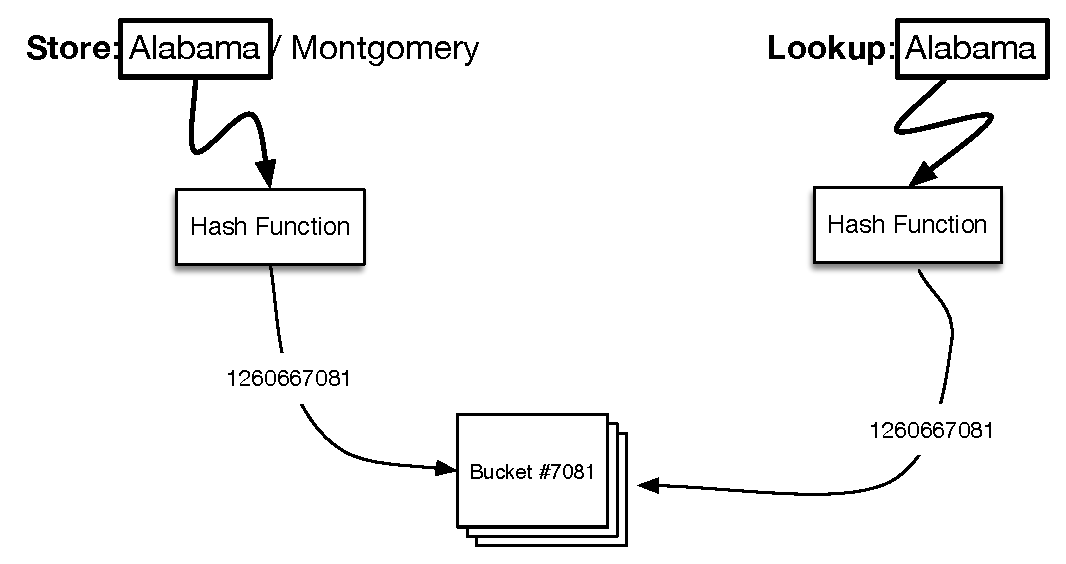
\includegraphics[scale=0.5]{images/hash-table-process.pdf}
\end{center}
\caption{Hash Table Storage and Retrieval}
\label{fig:hash-table-process}
\end{figure}

In our example, the keys were state names and the
values were their associated capitals. Using this hash
function, the key/value pairs can be assigned into 10 
buckets as seen in Table \ref{table:hash-table-state-capitals}.
As the table shows, the states are not spread out evenly into 
buckets. For example, bucket \#8 has
eight states, but bucket \#4 has only two. Keeping the same hash function but using 30 buckets
instead of 10 reduces this variability significantly. That's the advantage of keeping the hash
function separate from the desired number of buckets.

\begin{table}
\begin{center}
\begin{tabular}{r|p{4in}}
\textbf{Bucket} & \textbf{State Capitals (Values)} \\
\hline
1 & (washington  olympia)  (utah  salt-lake-city)  \hfill\break (rhode-island  providence)  (new-hampshire  concord)  \hfill\break (minnesota  st-paul)  (kentucky  frankfort) \\
\hline
2 & (nebraska  lincoln) (louisiana  baton-rouge) \hfill\break  (hawaii  honolulu)  (alabama  montgomery) \\
\hline
3 & (pennsylvania  harrisburg)  (new-york  albany) \hfill\break  (new-mexico  santa-fe)  (maine  augusta) \hfill\break  (indiana  indianapolis)  (georgia  atlanta) \\
\hline
4 & (missouri  jefferson-city)  (colorado  denver) \\
\hline
5 & (oregon  salem)  (michigan  lansing) \hfill\break  (arkansas  little-rock)  (arizona  phoenix) \\
\hline
6 & (wisconsin  madison)  (new-jersey  trenton) \hfill\break  (kansas  topeka)  (florida  tallahassee) \hfill\break  (alaska  juneau) \\
\hline
7 & (wyoming  cheyenne)  (tennessee  nashville) \hfill\break  (south-dakota  pierre)  (oklahoma  oklahoma-city) \\
\hline
8 & (west-virginia  charleston)  (vermont  montpelier) \hfill\break  (south-carolina  columbia)  (ohio  columbus) \hfill\break  (nevada  carson-city)  (mississippi  jackson)  (idaho  boise)  (connecticut  hartford) \\
\hline
9 & (north-dakota  bismarck)  (montana  helena) \hfill\break  (massachusetts  boston)  (maryland  annapolis) \hfill\break  (iowa  des-moines)  (california  sacramento) \\
\hline
10 & (virginia  richmond)  (texas  austin) \hfill\break  (north-carolina  raleigh) \hfill\break  (illinois  springfield)  (delaware  dover) \\
\end{tabular}
\end{center}
\caption{Hash Table for State Capitals}
\label{table:hash-table-state-capitals}
\end{table}

\begin{ExerciseList}
\Exercise Consider the words ``age'', ``cage'', and ``cape''. Using the hash function that we 
defined in this chapter, compute the hash values of each word and decide which bucket the
words map to, assuming we have exactly ten buckets.

\Exercise Implement the function \texttt{cap-pos} in ACL2. Hint: Use the ACL2
documentation to browser to lookup the built-in functions \texttt{char-code}, \texttt{symbol-name},
and \texttt{coerce}.

\Exercise There are many websites in the Internet that contain lists of the most popular baby names
(\url{https://www.babycenter.com/top-baby-names-2017.htm}) or most popular words in the English
language (https://www.englishclub.com/vocabulary/common-words-100.htm). Pick one of these lists 
and explore how well or poorly our hash function works on this list. For example, suppose we have 
a hash table with 128 buckets. What is the longest bucket? What is the average length of a bucket?
What is the average length of a \emph{non-empty} bucket? Which one of these lengths do you think
is the best way to measure how well the hash function is working? Why do you believe that?
\end{ExerciseList}

\section{Some Applications}

Hash tables provide a very powerful and useful abstraction, so it
is no surprise that they are essentially all around us. Let's look
at some common examples.

The most obvious example has to do with function definitions. When
you run an ACL2 program (or in any other computer language), the
computer needs to access the definition of each of your functions.
For example, the computer needs to know the definition of 
\texttt{append} to compute the value of \texttt{(append '(a b) '(c d))}.
This is, of course, a very common task so it is essential that the
lookup operations be as fast as possible.

Hash tables offer a very natural solution. You can store the function
definitions in a hash table where the key is the name of the function
and the value is the definition. This is almost certainly the solution
that your computer uses. The only other viable alternative is to use a
tree, as in Chapter \ref{ch:search-trees}, but hash tables offer a
significant advantage. As the number of entries increases, the time 
needs to find the answer in a tree also increases, albeit slightly,
since it is proportional to the height of the tree.
However, the time required to perform a lookup operation in a hash table
is proportional to the size of the longest bucket, and that can be
minimized by having many buckets. So the time needed for a lookup 
operation is essentially constant for a hash table, little more than
the time required to compute the hash function.

So hash tables are used behind the scenes in computing all the time,
even as far back as when we defined our very first function. It turns
out that hash tables are also ubiquitous in many other aspects of
computing. For example, database systems are the original killer app of 
computing. Some of the earliest databases were used to keep track
of airline reservations, and now databases are used to store and
process everything including student records at a university,
transactions at every register in any Walmart, the 
cast members for every movie produced in Hollywood, and even to 
the medical records of every person throughout their entire life.
Governments and corporations use databases to store literally 
thousands of records related to each one of us.

So what exactly is a database system? At its core, a database system
manages one or more tables, and each table is made up of one or more
records consisting of several attributes. Think of a database table as a
spreadsheet, where each record corresponds to a row in the spreadsheet
and each column corresponds to an attribute. For example, a table
may have information about states and their capitals, so each database
record (or row in a spreadsheet) would have one attribute for the 
state name and another attribute for the capital.

It is common to design a database table in such a way that one of its
columns is sufficient to identify a single record. For example, a
table containing student records may use the column ``Student ID''
to identify each student. If you know a student's ID, then the 
database system can find the one record for that student in the 
table. Part of the magic of database systems is that they can retrieve
that record from the table very quickly using specialized data
structures called \emph{database indexes}. In fact, the database
system uses indexes to retrieve a specific record quickly, even 
though the table may consist of millions of records that are stored 
in separate files on a disk drive.

So what, exactly, is a database index? In reality, database systems
offer many different types of indexes, but two types of indexes are
the most common. As you may have guessed, these common indexes
are hash-based indexes and tree-based indexes. In a sense, a database
table is a key/value pair, where the key is the column that is
sufficient to identify a single record and the value is the entire
record.

It turns out that hash-based indexes and tree-based indexes are
almost identical to the hash tables and trees that we have been
studying in the past two chapters. The only substantial difference
is that our trees and hash tables are ACL2 objects that are meant
to reside in a computer's memory, whereas the corresponding database
indexes are designed to retrieve records that may be stored in
potentially very large files.

But database systems go beyond simply storing and retrieving records
using a key. They also excel at finding information by combining
records in different tables. For instance, one table may have 
information regarding a student's permanent address and another table
may have information listing the students enrolled in any given course.
A database \emph{query} can combine these tables to find the states
represented in any given course, perhaps showing that students in a
region of the country are more likely than those in another region to
enroll in history courses. That's precisely the sort of insight that
data scientists find so valuable.

But this type of analysis can be prohibitively expensive. The simplest
way to combine the tables regarding student information and course
enrollment information is to consider all possible pairs. For example,
you could look at each course at a time, and for each course consider 
all the students who could be enrolled in it. At a mid-sized university
with 13,000 students and 80,000 enrollment records, that would require 
looking at 1,040,000,000 possible combinations---over a billion!

Hash tables provide a simpler alternative. The student information table
and the course enrollment information are combined using the student ID.
So before combining these tables, it is advantageous to hash both of them
using the student ID. Once this is done, each bucket contains some entries
from the student table and some from the course enrollment table. The entries
in each bucket must be considered exhaustively, but the total amount of
work is much smaller. To see this, suppose that there are 1,000 buckets, so
each has an average of 13 students and 80 courses. So to process each bucket 
requires 1,040 combinations, for a total of 1,040,000 combinations. That's
a thousand-fold improvement over the more direct approach.

The reason that hash tables work so well in this context is that they take
a single very large problem and turn it into many smaller problems. Instead
of combining two tables of size 13,000 and 80,000, you can combine 1,000
tables of size 13 and 80. This savings is significant in itself, but it can
be even more dramatic if the smaller problems can be performed in different
computers. For example, if you have 1,000 computers, each one of them can be
working on a different bucket, so the total time to find the answer is 
just the time to consider 1,040 combinations, or a million-fold improvement
over the direct approach! This is exactly the sort of thing that companies
with very large databases do---companies like Google, Facebook, and Amazon,
for example. They use thousands of computers to process the databases, and
hash tables are the key to spreading the work evenly across all those
machines.

Before concluding this chapter, we want to tell you about another important
application, this time just of hash functions instead of hash tables. Suppose
that we were to send you a very large file. After waiting a few hours 
for the file to transfer to your computer, how do you know that the file 
transferred correctly? It is possible, after all, that one of the characters
in the file was changed by a network glitch. Or perhaps a prankster interposed
himself between us and arranged to give you a false copy of the file.

You've probably guessed that hash functions are the answer to this problem.
Before sending you the file, we could use a hash function to compute a hash
value for the file. After you receive it, you would use the same hash function
to create a hash value, and then you can compare those hash values to make sure
they're identical. While it is \emph{possible} that two files end up with the 
same hash value, if we use a good hash function, it would be extremely unlikely. 
Variations of this idea are behind digital signatures, and sophisticated 
algorithms that keep multiple copies of a file synchronized with one another.
Hash functions and hash tables really are central to practical computing at
large scale. We'll consider more aspects of large-scale, practical computing 
in the next part of this book.

%%% Local Variables:
%%% mode: latex
%%% TeX-master: "book"
%%% End:
